%-----------------------------------LICENSE------------------------------------%
%   This file is part of tikz_figures.                                         %
%                                                                              %
%   tikz_figures is free software: you can redistribute it and/or              %
%   modify it it under the terms of the GNU General Public License as          %
%   published by the Free Software Foundation, either version 3 of the         %
%   License, or (at your option) any later version.                            %
%                                                                              %
%   tikz_figures is distributed in the hope that it will be useful,            %
%   but WITHOUT ANY WARRANTY; without even the implied warranty of             %
%   MERCHANTABILITY or FITNESS FOR A PARTICULAR PURPOSE.  See the              %
%   GNU General Public License for more details.                               %
%                                                                              %
%   You should have received a copy of the GNU General Public License along    %
%   with tikz_figures.  If not, see <https://www.gnu.org/licenses/>.           %
%------------------------------------------------------------------------------%

% Use the standalone class for displaying the tikz image on a small PDF.
\documentclass[crop, tikz]{standalone}

% Import the tikz package to use for the drawing.
\usepackage{tikz}

% Tikz libraries used in the drawing.
\usetikzlibrary{hobby}

% Begin the document.
\begin{document}

    % Draw the figure.
    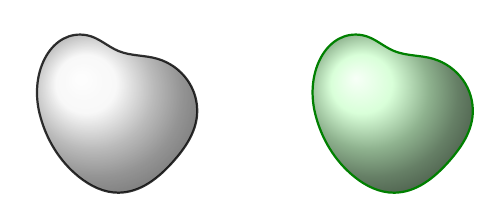
\begin{tikzpicture}[line width = 1pt]

        % Coordinates for the first blob.
        \coordinate (a) at (-4.0, 0.0);
        \coordinate (b) at (-4.5, 0.2);
        \coordinate (c) at (-5.0, 1.0);
        \coordinate (d) at (-4.4, 2.0);
        \coordinate (e) at (-4.0, 1.8);
        \coordinate (f) at (-3.5, 1.7);
        \coordinate (g) at (-3.0, 1.0);
        \coordinate (h) at (-3.3, 0.4);

        % Coordinates for the second blob, shift of the first.
        \coordinate (A) at (-0.5, 0.0);
        \coordinate (B) at (-1.0, 0.2);
        \coordinate (C) at (-1.5, 1.0);
        \coordinate (D) at (-0.9, 2.0);
        \coordinate (E) at (-0.5, 1.8);
        \coordinate (F) at (0.0, 1.7);
        \coordinate (G) at (0.5, 1.0);
        \coordinate (H) at (0.2, 0.4);
        \node at (0,1) (i) {$X$};

        % Draw the first blob using a Hobby curve.
        \path[%
            draw,
            thick,
            use Hobby shortcut,
            closed = true,
            ball color = gray!10!white,
            opacity = 0.8
        ] (a) .. (b) .. (c) .. (d) .. (e) .. (f) .. (g) .. (h);

        % We can use filldraw as well.
        \filldraw[%
            thick,
            use Hobby shortcut,
            closed = true,
            ball color = green!20!white,
            draw = green!50!black
        ] (A) .. (B) .. (C) .. (D) .. (E) .. (F) .. (G) .. (H);
    \end{tikzpicture}
\end{document}
